
% JuliaCon proceedings template
\documentclass{juliacon}
\usepackage{amsmath}

\setcounter{page}{1}

\begin{document}

% **************GENERATED FILE, DO NOT EDIT**************

\title{My JuliaCon proceeding}

\author[1]{1st author}
\author[1, 2]{2nd author}
\author[2]{3rd author}
\affil[1]{University}
\affil[2]{National Lab}

\keywords{Julia, Optimization, Game theory, Compiler}

\hypersetup{
pdftitle = {My JuliaCon proceeding},
pdfsubject = {JuliaCon 2019 Proceedings},
pdfauthor = {1st author, 2nd author, 3rd author},
pdfkeywords = {Julia, Optimization, Game theory, Compiler},
}



\maketitle

\begin{abstract}

Currently, more than 30 Rosenbrock-type methods are implemented in the widely used Julia package \verb|OrdinaryDiffEq.jl|.  
We discuss the differences and similarities of the various methods and explain why there is room for further improvements.
In particular, this concerns the solution of time dependent algebraic equations and continuous output within the solution of DAE problems. 
We present new methods \verb|Rodas23W| and \verb|Rodas3P| that are equipped with an error control of the interpolation.
We compare this approach with alternative concepts such as residual control and modification of the stiffly accurate embedded method of \verb|Rodas5P|, perform some 
benchmarks and present an application in the field of energy network simulation. 

\end{abstract}

\section{Rosenbrock-type methods}
We consider Rosenbrock-type methods for initial value problems of type
\begin{equation}
M \, y' = f(t,y) \, , \; y(t_0)=y_0 \, . \label{eq:dae} 
\end{equation}
These problems include systems of ordinary differential equations (ODEs) and in case of singular matrix $M$, systems of differential-algebraic equations (DAEs).
In the second case we assume that the DAE system has the index one.
When we can split (\ref{eq:dae}) into
\begin{eqnarray}
y' &=& f(t,y,z) \, , \label{eq:dae1} \\
0 &=& g(t,y,z) \, , \label{eq:dae2} 
\end{eqnarray}
the matrix $g_z = \frac{\partial g}{\partial z}$ must be non singular.
We refer further to \cite{hairer} for the index definition.

Rosenbrock-Wanner (ROW) methods for problems of type (\ref{eq:dae}) are defined by
\begin{align}
(M - h \, \gamma \, f_y) k_i &= h f(t_0+ \alpha_i h, y_0 + \sum_{j=1}^{i-1} \alpha_{ij} k_j) 
\nonumber \\ &
+ h \, f_y \sum_{j=1}^{i-1} \gamma_{ij}  k_j + h^2 \gamma_i f_t , \label{eq_row1} % \\
\end{align}
\begin{align}
y_1 &= y_0 + \sum_{i=1}^{s} b_i k_i,  \label{eq_row2} \quad \\
& \mbox{with} \quad f_y = \frac{\partial f}{\partial y}(t_0,y_0) \; , \quad f_t = \frac{\partial f}{\partial t}(t_0,y_0) \, . \nonumber
\end{align}
$h$ is the stepsize and $y_1$ is the approximation of the solution $y(t_0+h)$.
The coefficients of the method are $\gamma$, $\alpha_{ij}$, $\gamma_{ij}$, and $b_i$ define the weights. Moreover, it holds $\alpha_i = \sum_{j=1}^{i-1} \alpha_{ij}$ and
$\gamma_i = \gamma + \sum_{j=1}^{i-1} \gamma_{ij}$.\\

The theory of these methods is described very well in the books of Hairer, Wanner \cite{hairer} and Strehmel, Weiner, Podhaisky \cite{strehmel}, 
a good overview of the development of the methods since the 1960s is given by Lang \cite{lang}.

One disadvantage of ROW methods is that a new Jacobian matrix $f_y$ must be calculated at each time step.
A key reason for the efficiency of the methods in Julia is the calculation of the Jacobian with automatic differentiation.

To reduce the number of evaluations of the Jacobian, so-called Rosenbrock-W methods were introduced in \cite{steihaug}. 
These use an approximation of the Jacobian and can therefore be more efficient.
While some W methods are known for ODEs, such methods are difficult to derive for DAEs. Jax \cite{jax2} showed that for DAEs of index one the number of order conditions 
to be fulfilled is considerable. For a method of order 3, for example, 26 order conditions must be fulfilled. 
%Jax was able to determine a method of order $p=3$ with $s=7$ stages. 
The derivatives $g_z$ of the algebraic equations contained in (\ref{eq:dae2}) must nevertheless be exact, or at least keep to the error order 
$\mathcal{O}(h)$. 
%In order to limit the number of stages, we therefore only consider Rosenbrock-W methods for DAEs up to the order $p=2$.
For this reason, the most common W methods currently have a maximum order of two for DAEs.

The largest collection of implemented Rosenbrock-type methods is certainly contained in the Julia package \texttt{OrdinaryDiffEq.jl}, which is part of 
\texttt{DifferentialEquations.jl} developed by Rackauckas and Nie \cite{julia}.
Table \ref{tab:overview} summarizes the characteristics of the currently implemented schemes.

\begin{table*}[t] 
\tbl{Rosenbrock-type methods within \texttt{OrdinaryDiffEq.jl} and their properties.}{
%\begin{table}\label{tab:overview}
\begin{tabular}{r|ccccccccc}
Method & Ref. & $s$ & ODE & W & DAE & Para & A& $R(\infty)$ & Cont \\
\hline
GRK4T &\cite{kaps} 1979&4&4(3)&-&2(-)&2(-)&-&0.45(2.6)&- \\
GRK4A &\cite{kaps} 1979&4&4(3)&-&2(2)&2(2)&x&0.99(0.31)&- \\
RosShamp4 &\cite{shamp} 1982&4&4(3)&-&2(2)&2(2)&x&0.33(1.0)&- \\
Veldd4 &\cite{veld} 1984&4&4(3)&-&2(-)&2(-)&-&0.24(2.6)& -\\
Velds4 &\cite{veld} 1984&4&4(3)&2/-&2(2)&2(2)&x&0.33(0.33)& -\\
Scholz4\_7 &\cite{scholz} 1989&3&3(1)&-&3(2)&3(2)&x&0.73(0.52)&- \\
Ros4LStab &\cite{hairer} 1991&4&4(3)&-&2(2)&2(2)&x&0.0(0.55)& -\\
Rodas4 &\cite{hairer} 1991&6&4(3)&-&4(3)&2(2)&x&0.0(0.0)&x \\
Rodas42 &\cite{hairer} 1991&6&4(3)&-&4(3)&2(2)&x&0.0(0.0)&x \\
Rodas5 &\cite{rodas5} 1993&8&5(4)&-&5(4)&2(2)& x&0.0(0.0)&x \\
Rodas4P &\cite{rodas4p} 1995&6&4(3)&-&4(3)&4(3)&x&0.0(0.0)&x \\
ROS3 &\cite{rodas3} 1997&3&3(2)&-&2(2)&2(2)&x&0.0(0.5)& -\\
Rodas3 &\cite{rodas3} 1997&4&3(2)&-&3(2)&2(2)&x&0.0(0.0)&- \\
Rosenbrock23 &\cite{shampine} 1997&3&2(3)&2/-&2(-)&2(-)&x&0.0(1.6)& x\\
Rosenbrock32 &\cite{shampine} 1997&3&3(2)&2/-&-(2)&-(2)&-&1.6(0.0)& x\\
ROS3P &\cite{lang2} 2001&3&3(2)&-&3(2)&3(2)&x&0.73(0.73)&- \\
ROS34PW1a &\cite{ranga} 2005&4&3(2)&3/-&3(2)&3(2)&x&0.0(0.0)&- \\
ROS34PW1b &\cite{ranga} 2005&4&3(2)&3/-&3(2)&3(2)&x&0.0(0.0)&- \\
ROS34PW2 &\cite{ranga} 2005&4&3(2)&3/2&3(2)&3(2)&x&0.0(0.48)&- \\ %-- + W2 DAE
ROS34PW3 &\cite{ranga} 2005&4&4(2)&3/-&3(2)&3(2)&x&0.63(0.43)&- \\
ROS2S &\cite{rang12} 2012&3&2(1)&2/-&2(2)&2(1)&x&0.0(0.33)&- \\
ROS2PR &\cite{rang12a} 2012&3&2(1)&-&2(2)&2(1)&x&0.0(0.0)&- \\
ROS34PRw &\cite{rang12a} 2012&4&3(2)&3/2&3(2)&3(2)&x&0.0(0.25)&- \\ %-- + W2 DAE
ROS3PR &\cite{rang1} 2014 &3& 3(2)&-&3(2)&3(2)&x&0.73(0.73)& -\\
ROS3PRL &\cite{rang1} 2014&4&3(2)&-&3(2)&3(2)&x&0.0(0.25)&- \\
ROS3PRL2 &\cite{rang15} 2015&4&3(2)&-&3(2)&3(2)&x&0.0(0.25)&- \\
Rodas4P2 &\cite{rodas4p2} 2020&6&4(3)&2/2&4(3)&4(3)&x&0.0(0.0)&x \\ %-- W2 DAE
Rodas5P &\cite{rodas5p} 2023&8&5(4)&2/2&5(4)&4(4)& x&0.0(0.0)&x \\ %-- W2 DAE
\hline
Rodas23W &2024&5&2(3)&2/2&2(3)&2(3)&x&0.0(0.0)& x\\
Rodas3P  &2024&5&3(2)& - &3(2)&3(2)&x&0.0(0.0)& x\\
Rodas5Pe &2024&8&5(4)&2/2&5(3)&4(4)& x&0.0(0.46)&x \\ %-- W2 DAE
Rodas5Pr &2024&8&5(4)&2/2&5(4)&4(4)& x&0.0(0.0)&x \\ %-- W2 DAE
\hline 
\end{tabular}}
\label{tab:overview}
\begin{tabnote}
s = number of stages, order of convergence for ODEs, DAEs and parabolic problem (embedded
method in brackets), W = order of W method for ODEs / DAEs, A = A stable, $R(\infty)$ = limit of stablity function, Cont = continuous output for DAEs.\end{tabnote}
\end{table*}

Only the methods are specified which have a step size control. This is done using an embedded scheme with its own weights $\hat b_i$, such that 
\[ \hat y_1 = y_0 + \sum_{i=1}^{s} \hat b_i k_i\]
is an approximation of the solution with order $\hat p$.
The orders of the embedded method are shown in brackets in Table \ref{tab:overview}.

The stage number $s$ is a measure of the numerical effort per time step. For some methods, however, the number of function evaluations can also be less than $s$. 
This applies, for example, to the first five methods listed and is achieved by a clever choice of the coefficients $\alpha_{ij}$.

Roche \cite{roche} first considered ROW methods for DAEs and derived corresponding order conditions. 
Therefore, all methods before 1988 are only designed for stiff ODEs and achieve a maximum order of two for DAEs.
With \verb|Rodas4|, Hairer and Wanner \cite{hairer} then laid the foundation for a whole family of stiffly accurate methods for ODEs and DAEs. 
This property guarantees that the stability function $R(z)$ vanishes at infinity.
The stability function results when a method is applied to Dahlquist's test equation $y' = \lambda \, y$, $y(t_0)=y_0$. We obtain
$y_1 = R(z) y_0$ with $z = \lambda \cdot h$.
For A-stable methods $|R(z)| \leq 1$ must hold for all $z$ with $Re(z) \leq 0$. If in addition $\lim_{z \to \infty} R(z) = R(\infty)=0$, the method is called L-stable.
$|R(\infty)| < 1$ is also a requirement for the convergence concerning DAE problems.

With ODEs, the continuous output of the solution can simply be done using Hermite interpolation, because $y_0$, $y_0' = f(t_0,y_0)$, $y_1$, $y_1'=f(t_1,y_1)$ are known.
Ostermann \cite{ostermann} investigated the continuous extensions of Rosenbrock-type methods. All schemes of the \verb|Rodas| family (except \verb|Rodas3|) as well as  
\verb|Rosenbrock23/32| have their own interpolation, which is also suitable for DAEs.
If the matrix $M$ in (\ref{eq:dae}) is a diagonal matrix, a distinction can be made between differential and algebraic equations. 
In this case, all other methods use Hermite interpolation for the differential equations and linear interpolation for the algebraic equations.

W methods for ODEs were derived in particular by Rang (\verb|ROS34P| family), while W methods for DAEs are only available up to order 2. 
Currently, however, the W property is not utilized in the implementation, e.g. to reduce the number of evaluations of the Jacobian matrix.
However, it can be assumed that these methods are more suitable if the Jacobian matrix is approximated for example by finite differences and is therefore not exact.

Scholz \cite{scholz} investigated the order reduction of Rosenbrock methods. Further results were provided by Ostermann, Roche \cite{oro}, 
Lubich, Ostermann \cite{luos} and Rang \cite{rang2}.
There, the behavior of the methods for the Prothero-Robinson equation and semi-discretized parabolic problems were analyzed. 
Lang and Rang derived several methods (\verb|ROS3P| and \verb|ROS34P| family) that fulfill certain order conditions for the Prothero-Robinson equation. 
Methods \verb|Rodas4P|, \verb|Rodas4P2|, \verb|Rodas5P| are based on the additional conditons of Scholz.
Since order reductions for the Prothero-Robinson and parabolic problems are strongly related, we restrict ourselves to numerical investigations.
All methods were applied to the nonlinear parabolic problem (4.2) form \cite{rodas5p} with $n_x = 500$ space discretization points.
The numerical order obtained is shown in Table \ref{tab:overview}.

Although a variety of methods exist, there are applications that are not solved satisfactorily. This applies in particular to the continuous output of the 
solution for certain DAEs, which is discussed in Section \ref{sec:cont}.
This was the reason to derive new low order methods \verb|Rodas23W|, \verb|Rodas3P| (Section \ref{sec:construct}) and 
to implement two new variants of \verb|Rodas5P| (Section \ref{sec:rodas5pe}).
Finally, some benchmarks and applications are presented in Section \ref{sec:bench}.

\section{Continuous output for DAE problems} \label{sec:cont}

The first problem was discussed as an issue in the repository of\\ \verb|OrdinaryDiffEq|.
We consider the pure algebraic equation
\begin{equation} 0 = y_1 - \sin(20 \pi t) \; , \quad y_1(0)=0 \, .\label{eq:prob1} \end{equation}
Figures \ref{fig:dynamic} shows the numerical solution obtained with methods \verb|Rosenbrock23| and \verb|Rodas4|.
Here we see the following effects: With both methods, the time step control does not work, only seven time steps are required. 
However, the failure of the step size control has different causes. 

\verb|Rodas4| is a stiffly accurate method and its embedded scheme, too. Therefore, the solution of an algebraic equation like (\ref{eq:prob1}) is 
almost exact (see \cite{hairer}) and the difference between the fourth order and the embedded thrid order method does not provide any useful information for the 
step size control.
This applies regardless of the selected error tolerance.
The large step sizes make the third-order interpolation, which is integrated in the method, extremely inaccurate.
Of course, this can be avoided when a suitable bound for the maximum time step width $h_{max}$ is used. 
This example was the reason to issue a warning for the interpolation results when Rosenbrock methods are applied to pure algebraic equations.
Of course, this can easily be circumvented by adding a second equation $y_2'=0$. 
Therefore, it would be desirable to check not only the error of the solution at the discrete time steps but also the error of the interpolation.
Another possibility would be the modification of the embedded scheme so that it is no longer stiffly accurate.


With \verb|Rosenbrock23|, however, the solution at the discrete points in time is already completely wrong. 
The reason for this is that the third-order method used for step size control is not stable for DAEs. 
Figure \ref{fig:stability} shows the stability regions of the two second- and third-order methods. For the stability function of the third order method, $R(\infty) = 1.6 >1$ holds. 
Therefore, the error test is only applied internally to the differential variables. In order to prevent such large errors an
additional error test for the algebraic variables was introduced recently which controls the residuum $||f(t,y)||$ at the end of each timestep. 
Nevertheless the modification of (\ref{eq:prob1}) into the equivalent problem
\begin{equation}
\begin{pmatrix} 0&1\\0&1 \end{pmatrix}
\begin{pmatrix} y_1'\\y_2' \end{pmatrix} =
\begin{pmatrix} y_1 - \sin(20 \pi t) + 1 \\ 1 \end{pmatrix} , 
\begin{pmatrix} y_1(0)\\y_2(0) \end{pmatrix} = \begin{pmatrix} 0\\0 \end{pmatrix} 
 \label{eq:prob1a}
\end{equation}
leads to an error exit of the method due to instability and 
shows, that this measure dose not solve the inherent problem with \verb|Rosenbrock23|.

\begin{figure}[t]
\centerline{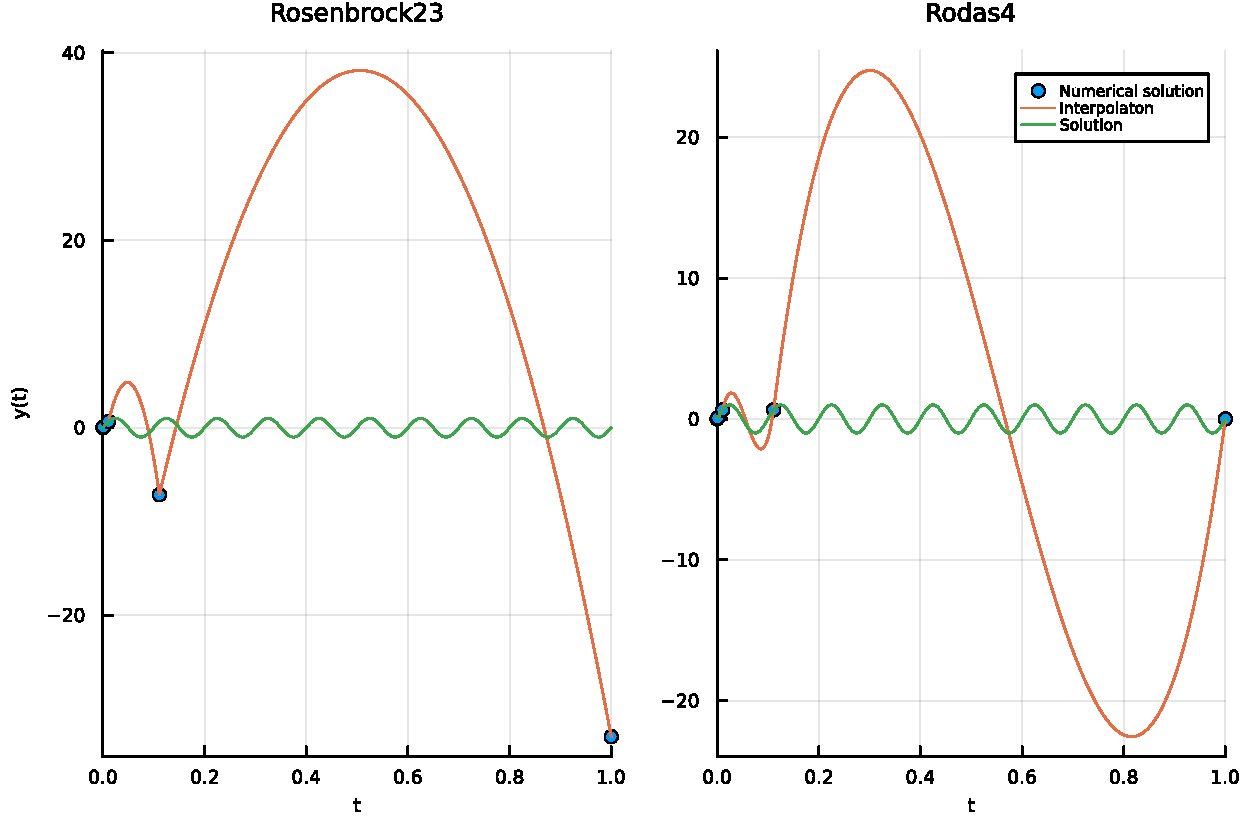
\includegraphics[width=0.47\textwidth]{Abb_1.pdf}}
\caption{Numerical and analytical solution of problem (\ref{eq:prob1}) with \tt Rosenbrock23 \rm and \tt Rodas4 \rm (OrdinaryDiffEq v6.40.1).}
\label{fig:dynamic}
\end{figure}

\begin{figure}[t]
 \centering
 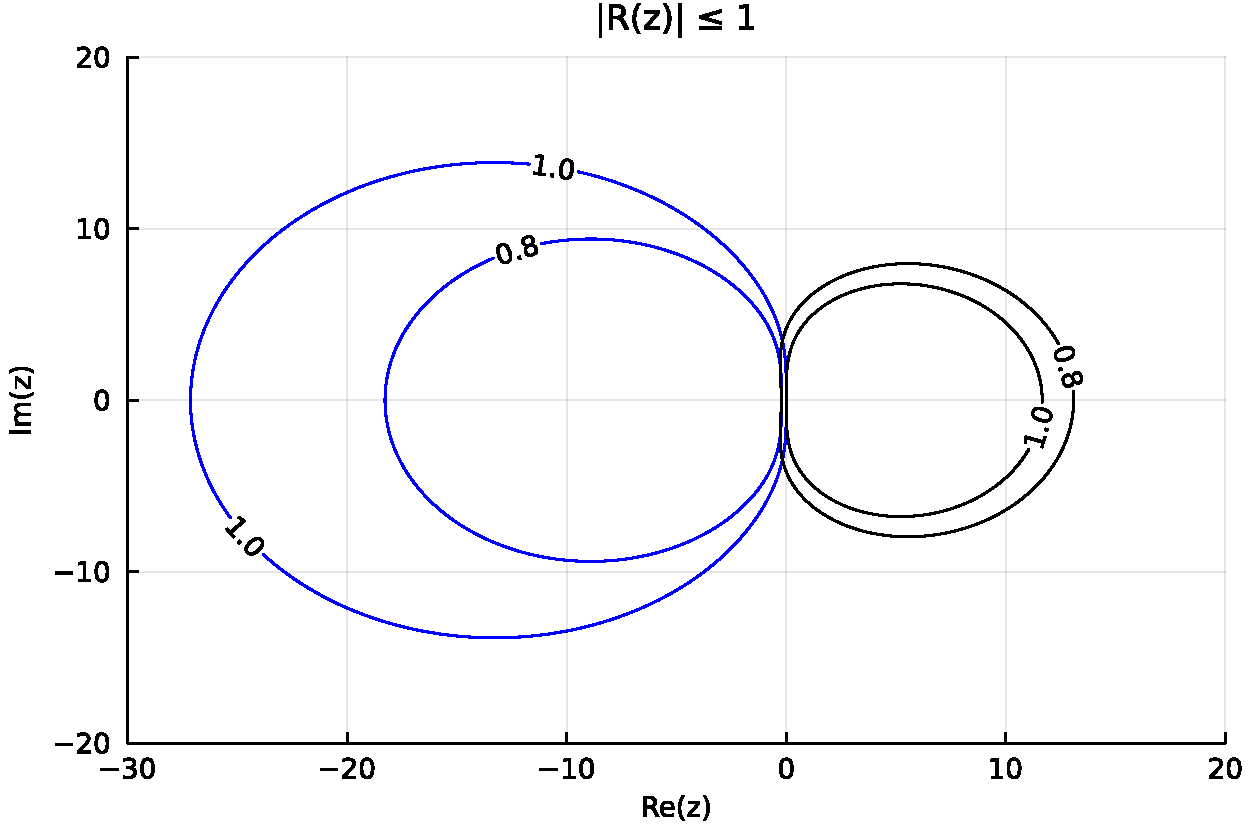
\includegraphics[width=0.45\textwidth]{stability_rosenbrock23.pdf}
 \caption{Stability regions of \tt Rosenbrock23\rm. Black method of order two, blue method of order three.}\label{fig:stability}
\end{figure}

Next, we tested all of the available Rosenbrock and Rosenbrock-W methods in \verb|DifferentialEquations.jl| on problem (\ref{eq:prob1a}).
All variants of \verb|Rodas4|, like \verb|Rodas42|, \verb|Rodas4P|, \verb|Rodas4P2|, \verb|Rodas5|, 
\verb|Rodas5P|, \verb|Rodas3| showed the same behaviour as illustrated in Figure \ref{fig:dynamic}.
Note, that \verb|Rodas3| has only a Hermite interpolation, which is not suited for DAEs.\\

\verb|Rosenbrock32| is the same method as \verb|Rosenbrock23|, but the 3rd order scheme is used for the solution, here. Therefore, it is 
unstable and not able to solve the problem.

All other methods are not equipped with their own interpolation. Since the mass matrix $M$ is not a diagonal matrix, 
it is not possible to distinguish between differential and algebraic equations and interpolation cannot be applied.
The following methods are only successful if the option \verb|dense=false| is used:
\verb|scholz4_7|, \verb|ROS2S|, \verb|ROS3|, \verb|ROS3P|,  \verb|ROS3PR|, \verb|ROS3PRL|, \verb|ROS3PRL2|, \verb|ROS34PW1a|, \verb|ROS34PW1b|, \verb|ROS34PW2|, 
\verb|ROS34PW3| and \verb|ROS34PRw|. 

The next example is a simple DAE problem:
\begin{eqnarray}
y_1' &=& -y_1  \; ,\label{eq:prob2_1}\\
0 &=& y_2 -(1-t^2)^4 \; .\label{eq:prob2_2}
\end{eqnarray}
For the initial values $y_1(0)=1$, $y_2(0)=1$ the solution is given by 
$y_1(t)= e^{-t}$, $y_2(t)=(1-t^2)^4$. We solve this system in the time interval $t \in [0,10]$ 
using different methods with different tolerances and show the work-precision diagram in Figure \ref{fig:bench1}.
The $L_2$-error shown is taken at 100 evenly spaced points via interpolation and should reflect the error of the dense output formulae.
\begin{figure}[t]
 \centering
 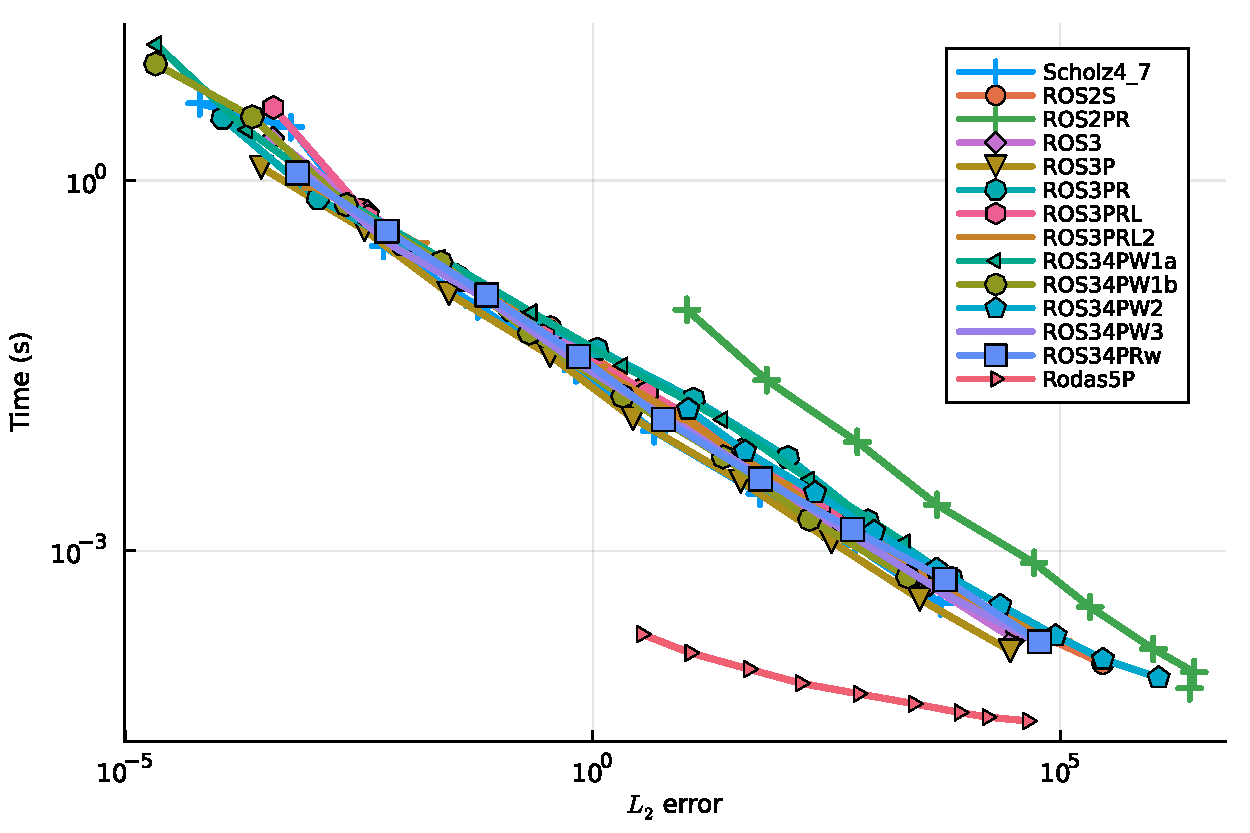
\includegraphics[width=0.47\textwidth]{Abb_2.pdf}
 \caption{Work-precision diagram for DAE system (\ref{eq:prob2_1},\ref{eq:prob2_2}).}\label{fig:bench1}
\end{figure}
We can see that almost all Rosenbrock methods used have a similar behavior. Only \verb|ROS2PR| requires significantly more computing time.
The reason for the similarities is the linear interpolation which is implemented for the algebraic variables.
On the other hand, we see that Rodas5P works much more efficiently, but achieves a considerably lower accuracy. 
The reason for the lower accuracy is again due to the stiffly accurate property of the \verb|Rodas| methods, which all behave similarly. 
Due to the almost exact solution of the algebraic equation, too large time steps are again used and the interpolation is inaccurate.
A comparison of the required time steps illustrates the characteristics of the different methods: 
With a tolerance of \verb|abstol=reltol=1.0e-8|, for example, \verb|ROS34PRw| requires 83070 time steps, whereas \verb|Rodas5P| requires only 52.
With \verb|Rosenbrock23| the solution was not possible within a reasonable computing time.


Therefore, the need for improved methods exists. We discuss three different approaches in Sctions \ref{sec:construct} and \ref{sec:rodas5pe}.

\section{Construction of Rodas23W / Rodas3P} \label{sec:construct}
First, we want an alternative for \verb|Rosenbrock23| that is often efficient for stiff ODEs, but not for DAEs.
A stiffly accurate method is desirable, but coupled with error control for the interpolation scheme. 
Moreover, the number of only three evaluations of the right hand side of (\ref{eq:dae}) should be preserved and the 
W property, so that an inexact Jacobian matrix may be used.
Our goal is to develop a \verb|Rodas23W| and \verb|Rodas3P| method. It is the same procedure, depending on which 
scheme is interpreted as an embedded method. 
\verb|Rodas23W| is of order $p=2$ with W property for DAEs, \verb|Rodas3P| is of order $p=3$ and is analogous 
to \verb|Rodas4P| particularly 
suitable for the Prothero-Robinson equation and semi-discretized parabolic problems.
Both methods have a dense-output formula of the same order. This makes it possible to check the errors of the 
interpolation and the problems that occurred in equation (\ref{eq:prob1}) can be avoided.

A method of order $p=3$ for index one DAEs of type (\ref{eq:dae}) must fulfill conditions No.1, 2, 3, 4, 5 of Table \ref{tab:conditions}, see \cite{hairer,roche}.
Here coefficients $\beta_{i}$ are given by $\beta_i = \sum_{j=1}^i \beta_{i j}$ with
$\beta_{i j}= \alpha_{i j} + \gamma_{i j}$ for $j < i$ and $\beta_{i i} = \gamma$.
When collecting coefficients $\beta_{ij}$ in matrix $B$, coefficients $w_{ij}$ arise from matrix $W = B^{-1}$.

If an inexact Jacobian $f_y$ or $f_t$ is to be used in equation (\ref{eq_row1}), additionally the W conditions must be considered.
Up to order $p=2$ these are conditions No.6, 7, 8 of Table  \ref{tab:conditions}.
No.7 and No.8 only apply, when DAEs are solved. Note, that nevertheless derivatives $g_z$ of the algebraic equations (\ref{eq:dae2}) with respect to the 
algebraic variables should be exact
or at least of error order $\mathcal{O}(h)$, see \cite{jax2}.
Condition No.9 guarantees convergence order $p=2$ for certain DAEs of index two, see \cite{lubich}.

To reduce order reduction, condition No.10 is taken into account. It is discussed in \cite{scholz,rodas5p} and
means, that in the stiff case order reduction for the Prothero-Robinson model is restricted to $p=2$ and for semi-discretized parabolic PDEs
order $p=3$ is preserved.

\begin{table} 
\tbl{Order conditions for methods {\tt Rodas23W} and {\tt Rodas3P}.}{
\begin{tabular}{rcccl}
%\hline
\hline\noalign{\smallskip}
No & & Order &  Condition \\
%\hline
\noalign{\smallskip}\hline\noalign{\smallskip}
  1& ODE & 1 & $\sum b_i = 1$\\
  2& ODE & 2 & $\sum b_i \beta_{i} = 1/2$\\
  3& ODE & 3 & $\sum b_i \alpha_{i}^2 = 1/3$\\
  4& ODE & 3 & $\sum b_i \beta_{ij} \beta_{j} = 1/6$\\
  5& DAE & 3 & $\sum b_i w_{ij} \alpha_{j}^2 =1$\\  
  \hline
  6& W ODE &2 & $\sum b_i \alpha_{i} = 1/2$ \\ 
  7& W DAE &2 & $\sum b_i \alpha_{ij} w_{jk} \alpha_{k} = 1/2$ \\
  8& W DAE &2 & $\sum b_i w_{ij} \alpha_{j} = 1$ \\
  9& Index-2&2& $\sum b_i w_{ij} w_{jk} \alpha_k^2= 2$ \\
 10& Prot-Rob&3   & $C_2(H)=\sum_{i=0}^s A_i H^i = 0$ \\
\noalign{\smallskip}\hline
\end{tabular}}
\label{tab:conditions}
\end{table}

Now, we want to construct a method of order $p=3$ with an embedded scheme of order $\hat p = 2$ and stages $\hat s = s-1$, fulfilling as many conditions as possible.
Both methods should be stiffly accurate. This leads to conditions $b_i = \beta_{s i}$ for $i=1,...,s$, $\hat b_i = \beta_{s-1,i}$ for $i=1,...,s-1$ and
$\alpha_s = \alpha_{s-1} = 1$.

Moreover, both methods should be equipped with interpolation formulas for dense output of the same order.
For interpolation between $y_0$ and $y_1$ we apply equations (\ref{eq:interp1}), (\ref{eq:interp2}), see \cite{hairer}.
\begin{eqnarray}
 y(t_0 + \tau \, h) &=& y_0 + \sum_{i=1}^s b_i(\tau) k_i \; , \quad \tau \in [0,1] \, ,\label{eq:interp1} \\
 b_i(\tau) &=& \tau (b_i-c_i) + \tau^2 (c_i-d_i) + \tau^3 d_i \, .\label{eq:interp2}
\end{eqnarray}
The computation of coeffcients $c_i$ and $d_i$, $i=1,...,s$ requires as many linear equations as order conditions are to be fulfilled. Thus
we need $s=5$ stages for a third order interpolation. In order to minimize
computational efforts per timestep, the number of function evaluations should be lower than the stagenumber $s=5$.

It turnes out that it is possible to derive a method \verb|Rodas3P| with embedded scheme \verb|Rodas23W| fulfilling the order conditions given in
Table \ref{tab:erfuellt}.

\begin{table} \label{tab:erfuellt}
\tbl{Fulfilled order conditions for methods {\tt Rodas23W} and {\tt Rodas3P} and its continuous output formulas.}{
\begin{tabular}{lcccccccccc}
\hline
 & 1 & 2 & 3 & 4 & 5 & 6 & 7 & 8 & 9 & 10 \\
\hline
Rodas3P &x&x&x&x&x& & &x&x&x \\
continuous output &x&x&x&x&x& & & & & \\
Rodas23W &x&x& & &x&x&x&x&x&x \\
continuous output&x&x& & &x&x& &x& &  \\
\hline
\end{tabular}}
\end{table}

The coefficients are shown in Table \ref{tab:coeff}.
As we can see from the $\alpha$ coefficients, only three evaluations of the right-hand side of the system (\ref{eq:dae}) are required.
oth methods are A stable, their stability regions are shown in Figure \ref{fig:stabrodas3p}.
If we need the maximum possible order, we use \verb|Rodas3P| and \verb|Rodas23W| as embedded methods for stepsize control. 
If we want to take advantage of the W properties, we can also proceed in exactly the opposite way.

\begin{table}
\tbl{Coefficients of {\tt Rodas23W}( $\hat{}$ ) and {\tt Rodas3P}.}{
\begin{minipage}{25pc}
\begin{eqnarray*}
\alpha &=& \begin{pmatrix} 
0 & 0 & 0 & 0 & 0 \\[0.2em]
\frac{4}{9} & 0 & 0 & 0 & 0 \\[0.2em]
0 & 0 & 0 & 0 & 0 \\[0.2em]
-\frac{217}{384} & \frac{183}{128} & \frac{13}{96} & 0 & 0 \\[0.2em]
-\frac{217}{384} & \frac{183}{128} & \frac{13}{96} & 0 & 0 \\
\end{pmatrix} , \;
\beta = \begin{pmatrix} 
\frac{1}{3} & 0 & 0 & 0 & 0 \\[0.2em]
0 & \frac{1}{3} & 0 & 0 & 0 \\[0.2em]
-\frac{1}{12} & \frac{3}{4} & \frac{1}{3} & 0 & 0 \\[0.2em]
\frac{3}{8} & \frac{3}{8} & -\frac{1}{12} & \frac{1}{3} & 0 \\[0.2em]
\frac{33}{8} & -\frac{27}{8} & -\frac{3}{4} & \frac{2}{3} & \frac{1}{3} 
\end{pmatrix}\, ,  \\
\gamma &=& \frac{1}{3} \; , \quad b_i = \beta_{5 i} \; , \quad \hat b_i = \beta_{4i} \, , \\
 c &=& (\frac{51}{4},-\frac{27}{2},-\frac{9}{4},\frac{8}{3},\frac{1}{3}) \, ; \; d = (-\frac{135}{8},\frac{135}{8},3,-3,0) \, , \\
\hat c &=& (-\frac{3}{8},-\frac{3}{8},\frac{1}{12},\frac{19}{30},\frac{1}{30}) \, ; \; \hat d = (0,0,0,0,0) \, . \
\end{eqnarray*}
\end{minipage}}
 \label{tab:coeff}
\end{table}

Because the interpolation formulas of both methods also have the order $p=3$ and $p=2$ respectively, we can check their errors, too. 
The difference $y(t_0+ \tau \, h) - \hat y(t_0 + \tau \, h)$ leads to a third order polynomial in $\tau$. Thus we can compute the maximum difference 
\[err_i = \max_{\tau \in [0,1]}|y_i(t_0+ \tau \, h) - \hat y_i(t_0 + \tau \, h)|\]
 for each component $y_i$ of the interpolated solution. Similar to the error control after each timestep we require 
 $err_i \leq abstol + reltol \,|y_i|$ and reduce the stepsize when this condition is violated.
 
\begin{figure}
 \centering
 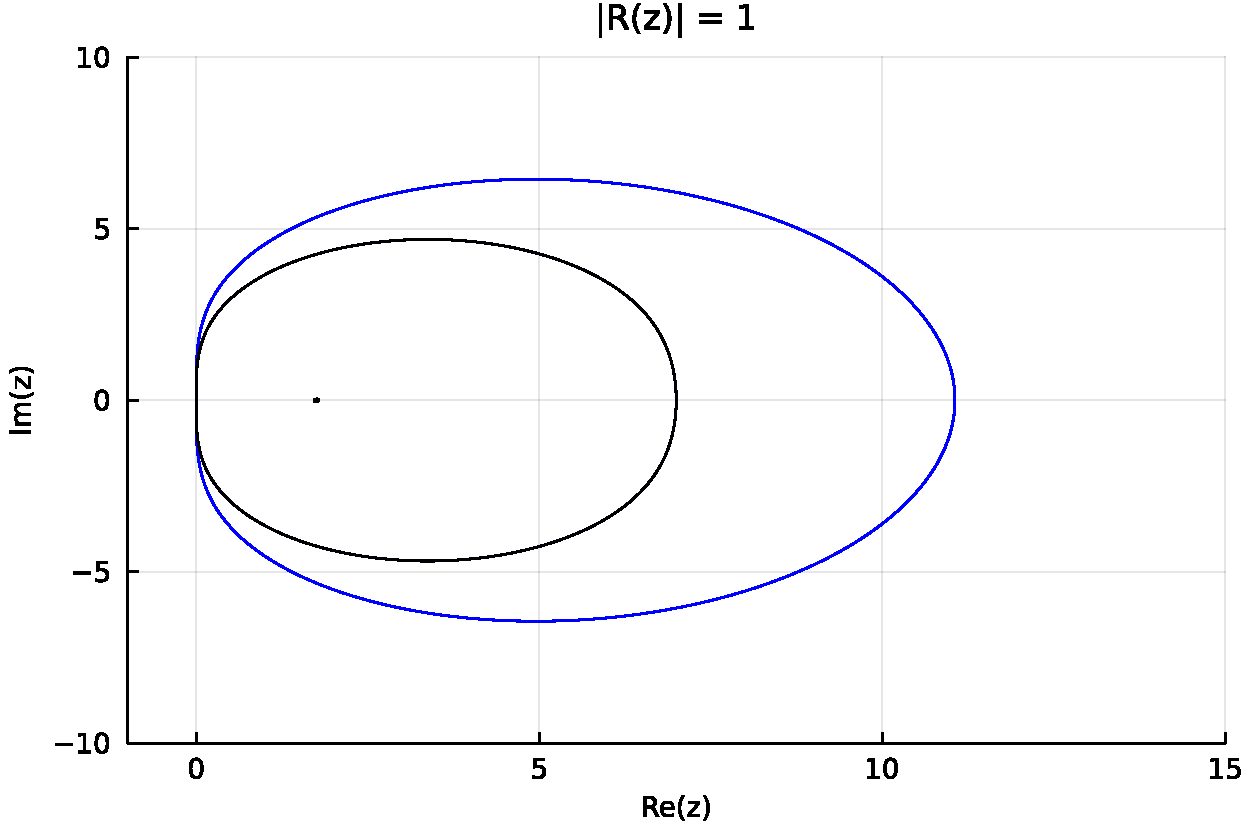
\includegraphics[width=0.45\textwidth]{stability_rodas3p.pdf}
 \caption{Stability regions of \tt Rodas3P \rm (black) and \tt Rodas23W \rm (blue).}\label{fig:stabrodas3p}
\end{figure}

\section{Residual control and modified embedded scheme for Rodas5P}\label{sec:rodas5pe}

Next we want to improve the higher order methods. We picked \verb|Rodas5P| because it is the most efficient method of the Rodas family in many cases.

First, we equip the method with an additional error test, which checks the residual of the interpolation in half of the step size.
With the help of the built-in interpolation of \verb|Rodas5P| we can calculate $y_{int}(t_0 + \frac{h}{2})$ and $y_{int}'(t_0 + \frac{h}{2})$ and 
determine the residual of (\ref{eq:dae}):
\[ res = ||M \, y_{int}'(t_0 + \frac{h}{2}) - f(t_0 + \frac{h}{2},y_{int}(t_0 + \frac{h}{2}))|| \, .\]
If $res$ is too large, the step size is reduced accordingly. As an error test, $res \leq abstol + reltol ||y_{int}(t_0 + \frac{h}{2})||$ has proven 
to be practicable. We call \verb|Rodas5P| together with this residual test \verb|Rodas5Pr|.
The additional calculation effort per step is limited to one extra function evaluation of the right-hand side of (\ref{eq:dae}).

Secondly, we change the embedded method so that it is no longer stiffly accurate. 
The embedded scheme of \verb|Rodas5P| has order $\hat p = 4$ and must fulfill 13 order conditions, see \cite{rodas5p}. 
For determining new coefficients $\hat b_1,...,\hat b_8$, $s=8$ degrees of freedom are available .
In order for these to differ from the previous ones, not all order conditions can be fulfilled. It is possible to compute new coefficients in such 
a way that only conditions (21),(22) from Table 3 in \cite{rodas5p} are not fulfilled. The new embedded method therefore has 
order $\hat p = 4$ for ODEs, but only $\hat p =3$ for DAEs. A-stability is preserved, but due to $\hat R(\infty)=0.46$, L-stability of the embedded scheme is lost.
This new method is called \verb|Rodas5Pe|.

\section{Benchmarks and applications} \label{sec:bench}

First, we consider problem (\ref{eq:prob1a}). Figure \ref{fig:bench1a} shows the work-precision diagram for the new methods. Again, the $L_2$ error is shown, which is strongly 
influenced by the interpolation. Here \verb|Rodas23W| delivers even better results than \verb|Rodas3P|. This is because \verb|Rodas23W| also fulfils the order condition No.5 
from Table \ref{tab:conditions}. \verb|Rodas5Pe| and \verb|Rodas5Pr| provide very similar results. The four new methods are the only ones that produce meaningful results for 
this problem with respect to the $L_2$ error.

\begin{figure}
 \centering
 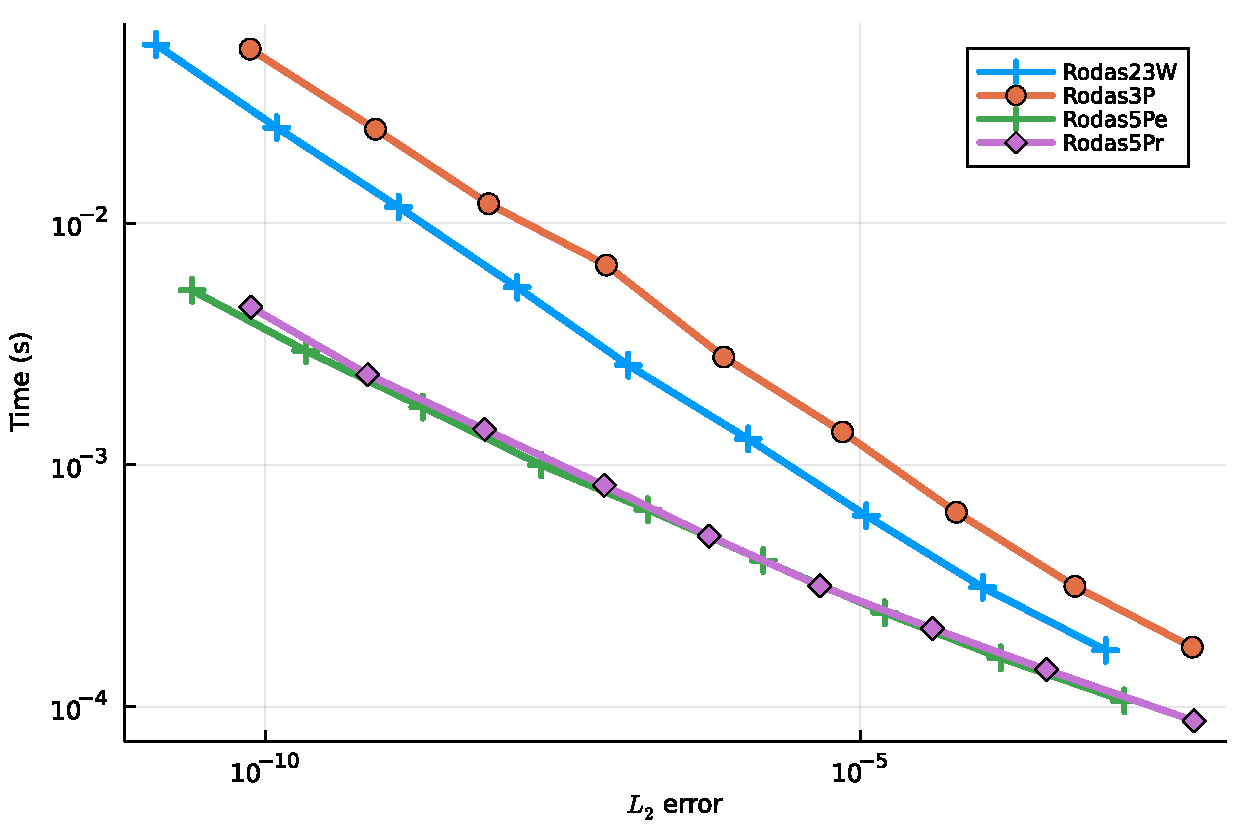
\includegraphics[width=0.47\textwidth]{Abb_1a.pdf}
 \caption{Work-precision diagram for DAE system (\ref{eq:prob1a}).}\label{fig:bench1a}
\end{figure}

Next, we consider problem (\ref{eq:prob2_1},\ref{eq:prob2_2}) and create a work-precision diagram analogous to Figure \ref{fig:bench1}. 
Figure \ref{fig:bench2a} shows that the accuracy is considerably improved by the new approaches and that the efficiency is significantly better 
than with all other Rosenbrock-type methods.

\begin{figure}
 \centering
 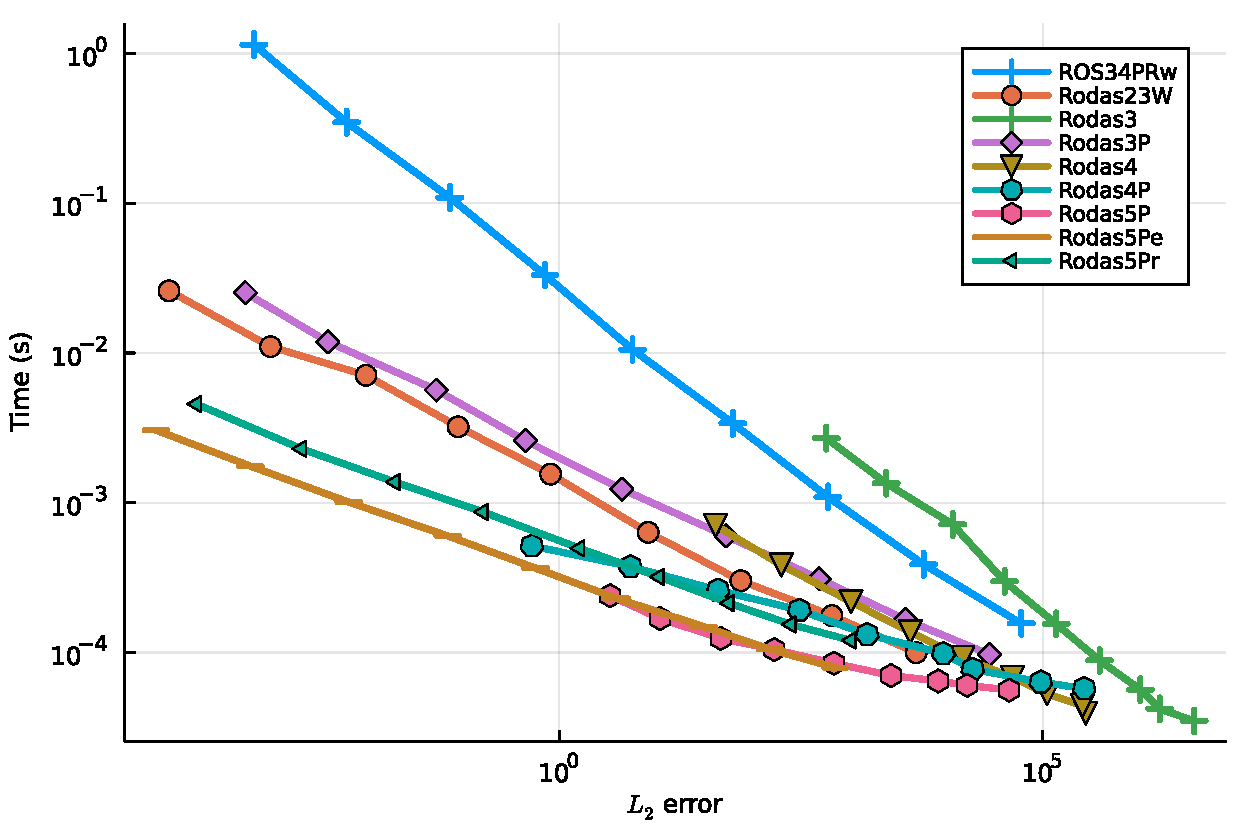
\includegraphics[width=0.47\textwidth]{Abb_2a.pdf}
 \caption{Work-precision diagram for DAE system (\ref{eq:prob2_1},\ref{eq:prob2_2}).}\label{fig:bench2a}
\end{figure}

Figure \ref{fig:bench3a} shows the results for a simple linear stiff ODE system
\begin{equation}
\begin{pmatrix} y_1'\\y_2'\\y_3' \end{pmatrix} =
\begin{pmatrix} -0.8 &12.5& 0\\ -12.5& -0.8& 0\\ 0& 0& -100 \end{pmatrix}
\begin{pmatrix} y_1\\y_2\\y_3 \end{pmatrix}   
%\begin{pmatrix} y_1(0)\\y_2(0)\\y_3(0) \end{pmatrix}=
%\begin{pmatrix} 0\\0\\0 \end{pmatrix}  . 
\label{eq:stiffode}
\end{equation}
with initial conditions $y_1(0)=y_2(0)=y_3(0)=0$.
Shown here is the $l_2$ error for $t \in [0,10]$, which does not include any interpolation results. The different orders of the Rodas methods are easy to distinguish and correspond to expectations. 
Why \verb|ROS3P|, \verb|ROS3PR|, \verb|ROS34PW1a| and \verb|ROS34PW1b| do not provide plausible results could not be clarified.

\begin{figure}
 \centering
 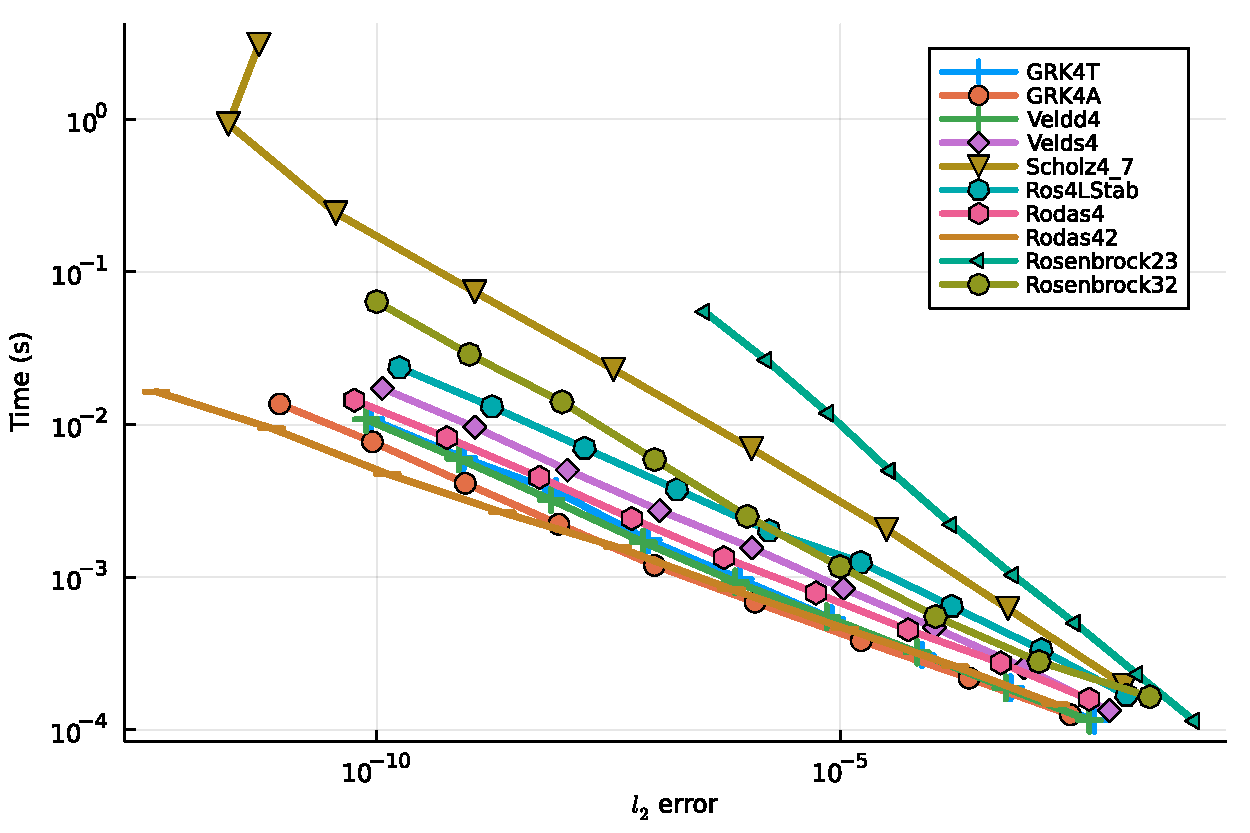
\includegraphics[width=0.47\textwidth]{Abb3a.pdf}
 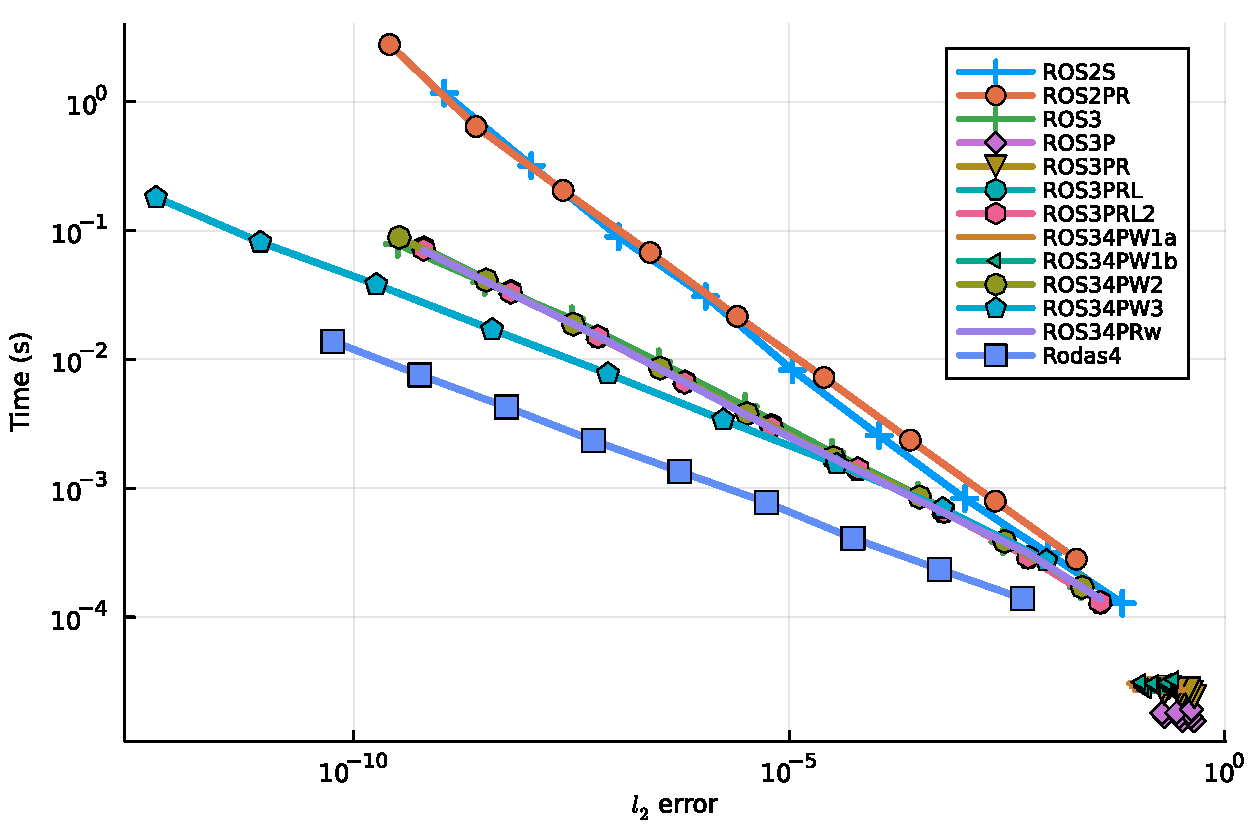
\includegraphics[width=0.47\textwidth]{Abb3b.pdf}
 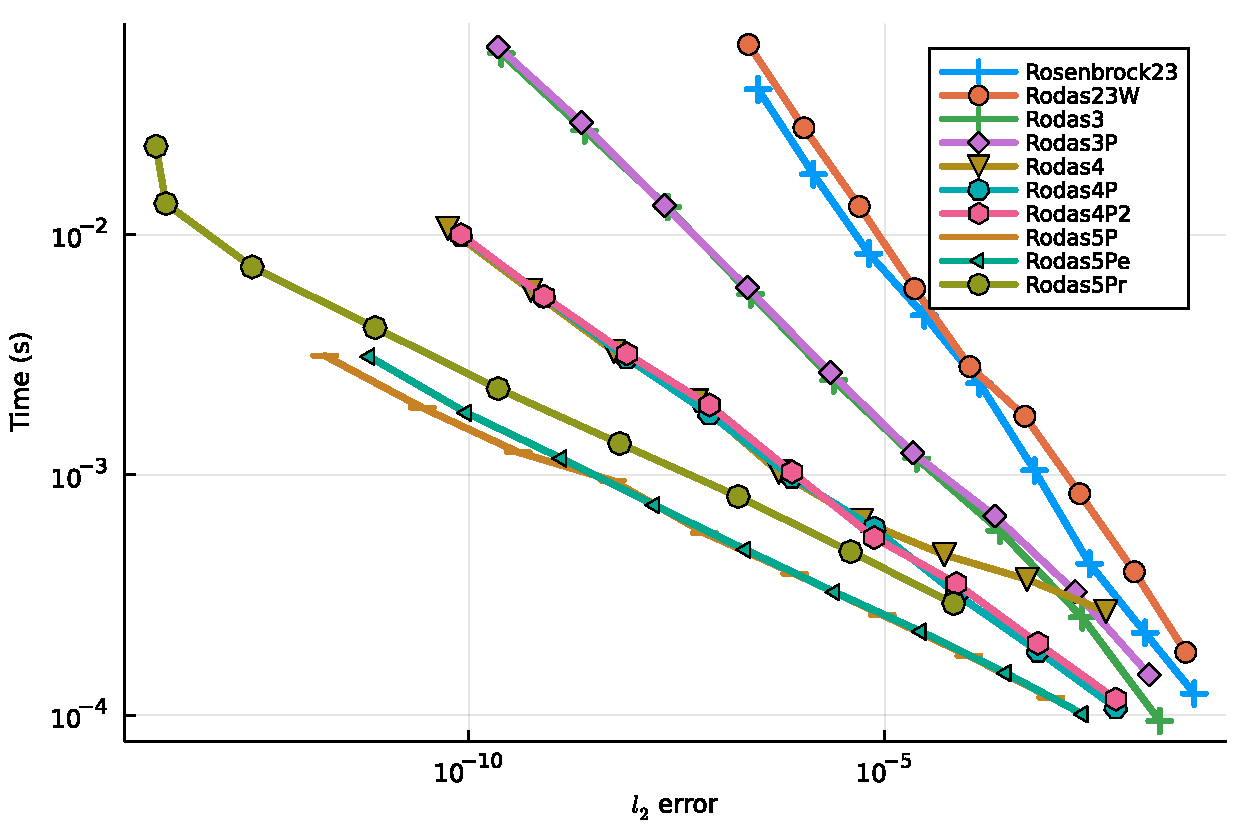
\includegraphics[width=0.47\textwidth]{Abb3c.pdf}
 \caption{Work-precision diagram for problem (\ref{eq:stiffode}).}\label{fig:bench3a}
\end{figure}

All procedures from Table \ref{tab:overview} that have the W property were applied to the following DAE system:
\begin{eqnarray}
y_1' &=& \frac{1}{2}y_2^3 y_3 \; , \label{eq:w1} \\
y_2' &=& \frac{1}{6} y_2 y_3 \; , \label{eq:w2}\\
0 &=& y_3 + \frac{6 y_1}{y_2^3} \; ,\label{eq:w3}
\end{eqnarray}
with $y_1(0) = y_2(0) =1$, $y_3(0)=-6$ and $t \in [0,1]$.
The Jacobian matrix was evaluated at time $t=0$ and kept constant. It should be noted that the derivative of the algebraic equation with respect to 
$y_3$ is thus exact for all $t$.
The methods \verb|Rosenbrock23|, \verb|Rosenbrock32|, \verb|ROS2S|, \verb|ROS34PW1a|, \verb|ROS34PW1b| could not solve the problem in a reasonable time. 
The results of the other methods are shown in Figure \ref{fig:benchW}. Here, the convergence properties for W methods applied to DAEs given in 
Table \ref{tab:overview} are confirmed.

\begin{figure}
 \centering
 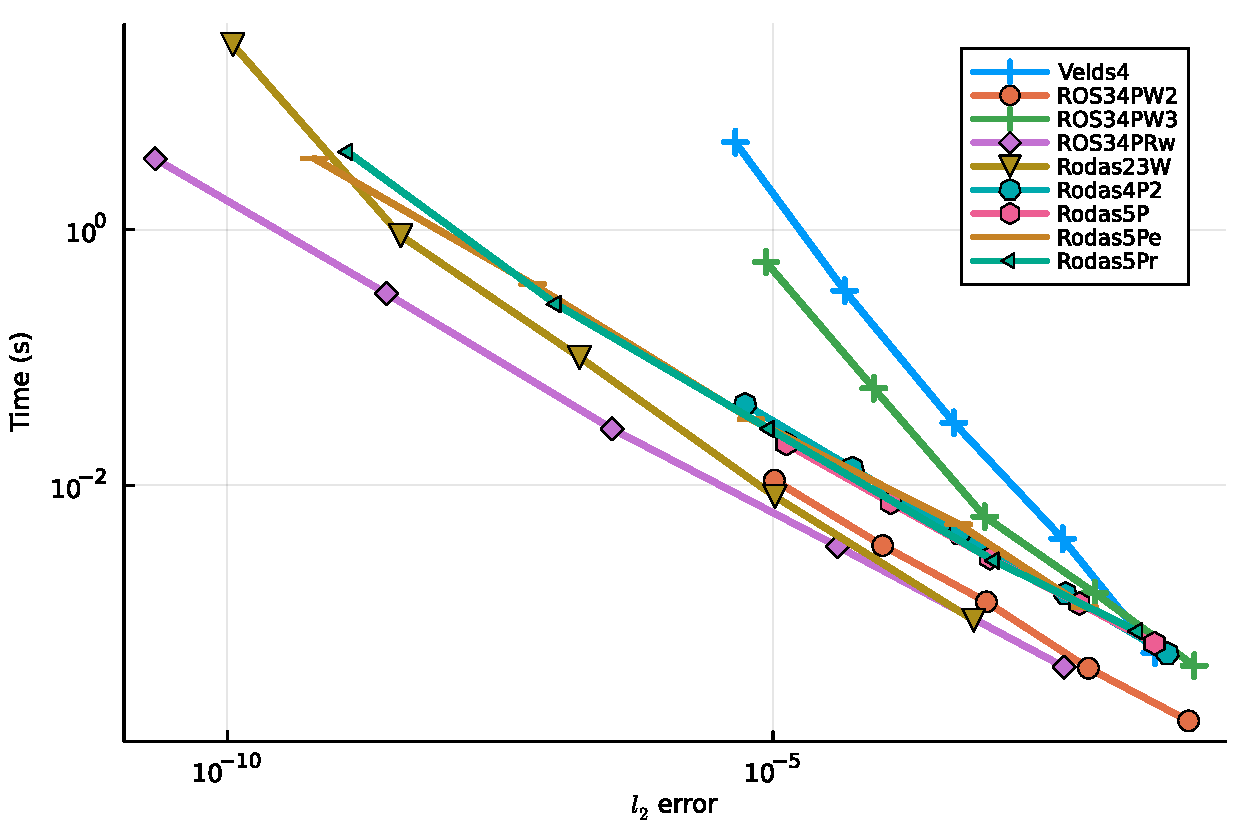
\includegraphics[width=0.47\textwidth]{Abb4.pdf}
 \caption{Work-precision diagram for problem (\ref{eq:w1},\ref{eq:w2},\ref{eq:w3}).}\label{fig:benchW}
\end{figure}

Finally, all 16 methods from Table \ref{tab:overview}, which have an order greater than two for parabolic problems, were applied to the  
nonlinear parabolic problem (4.2) presented in \cite{rodas5p}. The corresponding results using $n_x=500$ space discretization points are shown in Figure \ref{fig:benchpara}. 
This clearly shows the advantages of the \verb|Rodas4P|, \verb|Rodas4P2|, \verb|Rodas5P|, \verb|Rodas5Pe| and \verb|Rodas5Pr| methods in terms of efficiency. 
The accuracies achieved by the Rodas methods correspond to the specified tolerances $reltol = abstol \in [10^{-10},10^{-2}]$. 
The residual error control in \verb|Rodas5Pr| additionally increases the accuracy and is within the range of the other methods.

\begin{figure}
 \centering
 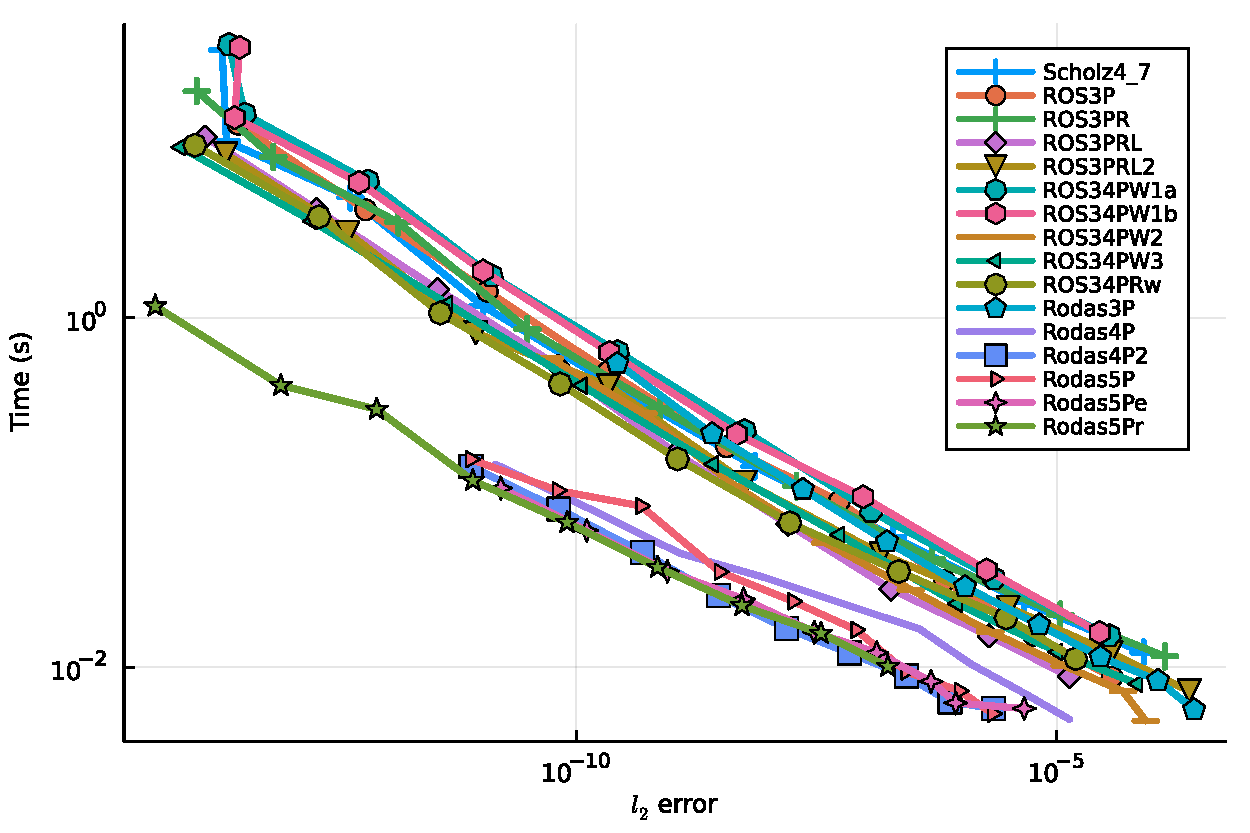
\includegraphics[width=0.47\textwidth]{Abb5.pdf}
 \caption{Work-precision diagram for parabolic problem (4.2) in \cite{rodas5}.}\label{fig:benchpara}
\end{figure}

Fortran, MATLAB and Julia Implementations of \verb|Rodas4P| respectively \verb|Rodas5P| have been used successfully in many applications concerning network simulation and are characterized in particular 
by their robustness, see \cite{jaxsteinebach,rentropsteinebach,ecmi,dreistadtsteinebach}.
Finally, we would like to show that the behavior shown in Figure \ref{fig:dynamic} may also occur in such real applications. 
For this purpose, we reduce the model presented in \cite{flexhyx} to a minimal demonstration network consisting of a battery, a photovoltaic feed-in and a consumer.
Figure \ref{fig:energy} shows the typical behavior over one day. The simulated state of charge of the battery is much smoother than the power of the 
photovoltaic and the consumer provided by measured time series. 

\begin{figure}
 \centering
 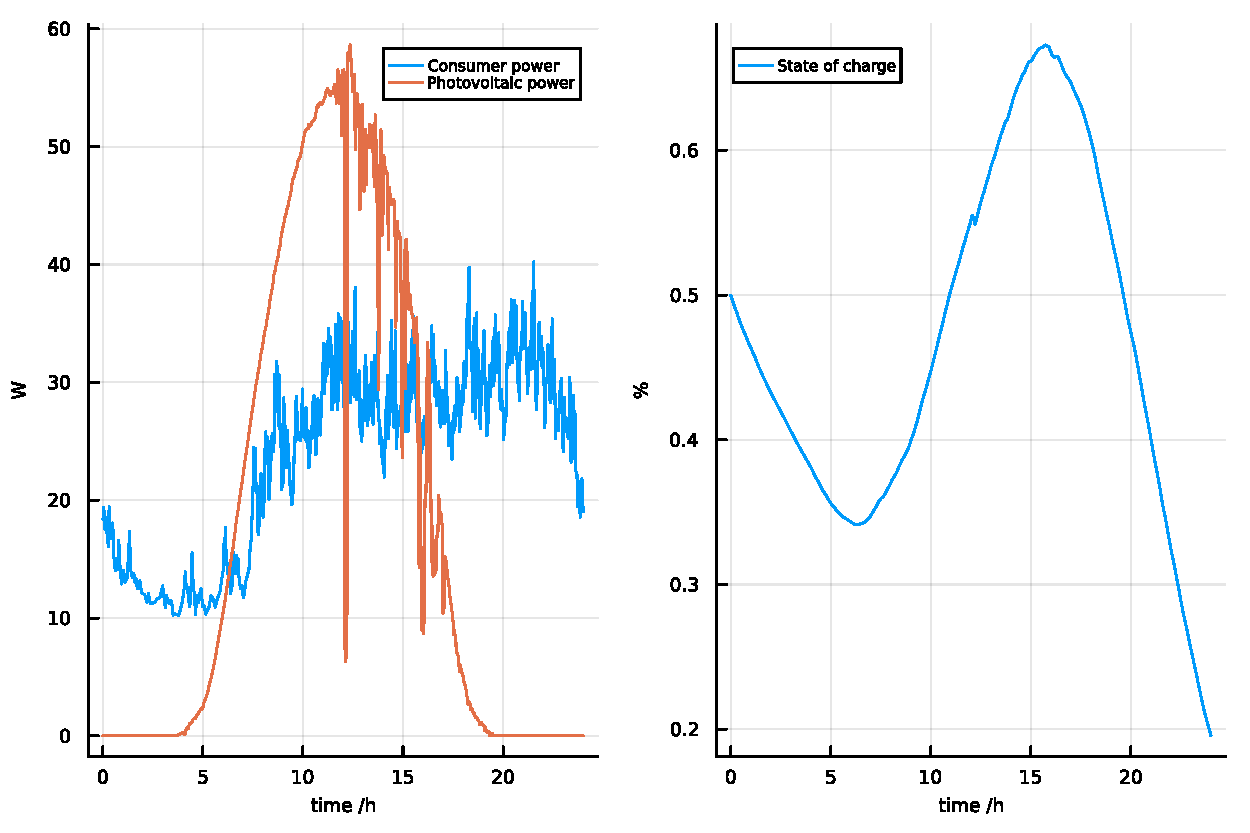
\includegraphics[width=0.47\textwidth]{Abb6a.pdf}
 \caption{Measured time series for photovoltaic and the consumer power and simulated state of charge of the battery.}\label{fig:energy}
\end{figure}

Typically, the energy network is modeled by a DAE system and algebraic equations of type $0 = I \cdot U - P(t)$ occur internally. $P(t)$ is the measured power and $I$, $U$ are time-dependent state 
variables for current and voltage.
Figure \ref{fig:energy1} shows that the dynamics of the input data is not fully resolved by the simulation using \verb|Rodas5P| due to time steps that are too large.
%It turns out that the input data of the model is not satisfactorily resolved by the simulation. 
The reason is the same as discussed in the example of equation (\ref{eq:prob1}).
The problem also occurs here because the remaining components of the network have a much smoother behavior than the input data.

\begin{figure}
 \centering
 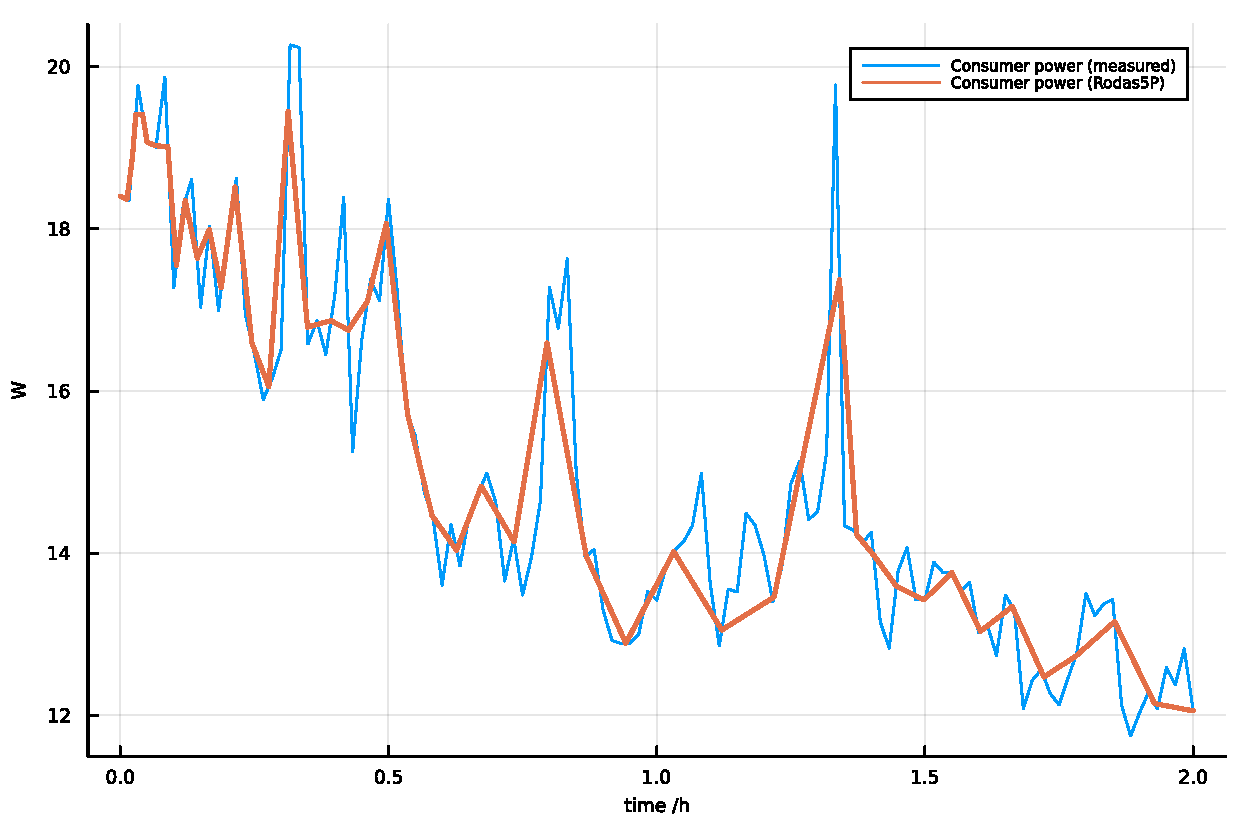
\includegraphics[width=0.47\textwidth]{Abb6b.pdf}
 \caption{Measured input data of the model and resolution generated by the simulation.}\label{fig:energy1}
\end{figure}

Table \ref{tab:battery} shows the solver statistics for the various methods of the Rodas family. A visual match of the curves shown in Figure \ref{fig:energy1} 
can only be observed when using the new methods \verb|Rodas23W|, \verb|Rodas3P|, \verb|Rodas5Pe|. 
This means, that at least around 10000 time steps are required.
All other methods show the same behavior as \verb|Rodas5P|, albeit to a lesser extent. For the residual control of \verb|Rodas5Pr| to be effective, 
the relative tolerance \verb|reltol| must be reduced slightly. For all results shown in Figure \ref{fig:energy1} and Table \ref{tab:battery}, \verb|abstol=reltol=1.0e-4| was chosen.

\begin{table} \label{tab:battery}
\tbl{Solver statistics for the simplified energy model.}{
\begin{tabular}{l|rrr}
\hline
& nfcn & nsucc & nfail \\
\hline
Rodas23W & 134172 &25043& 2985\\
Rodas3 &36417 &4679& 2085\\
Rodas3P & 134491 &25102& 2993\\
Rodas4 &60688 &6661& 1233\\
Rodas4P &53164 &5707& 1251\\
Rodas4P2 &44898 &4736& 1168\\
Rodas5 & 9856 &871& 143\\
Radas5P & 11628& 1013& 187 \\
Rodas5Pr & 12063 &983& 156 \\
Rodas5Pe & 112542 &9450& 2255\\
\hline
\end{tabular}}
\begin{tabnote}
$nsucc$ = number of successful time steps, 
 $nfail$ = number of rejected steps.
 \end{tabnote}
\end{table}

In conclusion, it can be summarized that with \verb|Rodas5Pe| and \verb|Rodas5Pr| two new variants of \verb|Rodas5P| are available. 
These can be used when time-dependent algebraic equations cannot be solved with sufficient resolution.
\verb|Rodas5Pe| uses an alternative embedded method that is not stiffly accurate, \verb|Rodas5Pr| is equipped with an error control for the residual of the interpolation. 
Alternatively, lower order methods can be applied, which are equipped with an error control by the second and third order interpolation schemes.
\verb|Rodas3P| has similar properties to \verb|Rodas4P|, \verb|Rodas5P| and \verb|Rodas23W| is preferable due to its W property if the Jacobian matrix is not exactly known.

%\newpage
\begin{thebibliography}{}

\bibitem{flexhyx} 
M.~Bareev-Rudy, S.~Meiswinkel, M.~Pfennig, S.~Schedler, B.~Schiffer, G.~Steinebach, T.~Clees,
Analysis of PtGtX Systems with Metal Hydride Storage Based on Coupled Electrochemical and Thermodynamic Simulation,
Energy Conversion and Management, submitted.
%Dec 8, 2023
%Conference Paper at 18th Conf. Sustainable Development of Energy, Water and Environment Systems, Dubrovnik (2023) 

\bibitem{hairer} E.~Hairer and G.~Wanner, Solving Ordinary Differential Equations II, Stiff and differential algebraic Problems, 
(2nd ed.), Springer-Verlag, Berlin Heidelberg (1996) 

\bibitem{rang12} A.~W. Hamkar, S.~Hartmann, J.~Rang, A stiffly accurate
Rosenbrock-type method of order 2. Appl. Num. Math., 62(12):1837–1848 (2012)

\bibitem{jax2} T.~Jax, A rooted-tree based derivation of ROW-type methods with arbitrary jacobian entries for solving index-one DAEs, 
Dissertation, University Wuppertal (2019)

\bibitem{jaxsteinebach}  
T.~Jax, G.~Steinebach,
Generalized ROW-Type Methods for Simulating Water Supply Networks,
In: Quintela, Barral et al. (Eds.): Progress in Industrial Mathematics at ECMI 2016, 19th European Conference on Mathematics for Industry, 
Springer, Cham,447-454 (2017). https://doi.org/10.1007/978-3-319-63082-3\_70 

\bibitem{kaps} P.~Kaps, P.~Rentrop, Generalized Runge-Kutta Methods of Order Four with Stepsize Control for Stiff Ordinary Differential 
Equations, Numerische Mathematik, 33, 55-68 (1979)

\bibitem{lang} J.~Lang, Rosenbrock-Wanner Methods: Construction and Mission, 
In: Jax T., Bartel A., Ehrhardt M., Günther M., Steinebach G. (eds) Rosenbrock—Wanner–Type Methods. Mathematics Online First Collections,
Springer, Cham., 1-17 (2021). https://doi.org/10.1007/978-3-030-76810-2\_2 

\bibitem{lang2} J.~Lang, J.G.~Verwer, ROS3P—An Accurate Third-Order Rosenbrock Solver Designed for Parabolic Problems, J. BIT Numerical Mathematics 41, 731–738 (2001). doi:10.1023/A:1021900219772

\bibitem{luos} C.~Lubich, A.~Ostermann, Linearly implicit time discretization of non-linear parabolic equations, 
IMA Journal of Numerical Analysis, 15(4), 555–583 (1995). https://doi.org/10.1093/imanum/15.4.555

\bibitem{lubich} C.~Lubich, M.~Roche, Rosenbrock methods for differential-algebraic systems with solution-dependent singular matrix multiplying the derivative,
Computing 43, 325–342 (1990). https://doi.org/10.1007/BF02241653

\bibitem{rodas5} G.~Di Marzo, RODAS5(4) – Méthodes de Rosenbrock d’ordre 5(4) adaptées aux problemes différentiels-algébriques. MSc mathematics thesis, Faculty of Science,
University of Geneva, Switzerland (1993)

\bibitem{ostermann} A.~Ostermann, Continuous extensions of Rosenbrock-type methods,  Computing 44, 59–68 (1990). https://doi.org/10.1007/BF02247965

\bibitem{oro} A.~Ostermann, M.~Roche, Rosenbrock methods for partial differential equations and fractional orders of convergence,
SIAM J. Numer. Anal. 30, 1084-1098 (1993)

\bibitem{julia} C.~Rackauckas, Q.~Nie, Differentialequations.jl--a performant and feature-rich ecosystem for solving differential equations in julia,
Journal of Open Research Software, 5(1), p.15, Ubiquity Press (2017)

\bibitem{ranga} J.~Rang, L.~Angermann,
New Rosenbrock W-methods of order 3 for partial differential algebraic equations of index 1, BIT 45, 761-787 (2005)

\bibitem{rang12a} J~Rang, An analysis of the Prothero–Robinson example for constructing new DIRK and ROW methods, Informatik-Bericht 2012-03, TU Braunschweig (2012)

\bibitem{rang1} J.~Rang, The Prothero and Robinson example: 
Convergence studies for Runge-Kutta and Rosenbrock-Wanner methods, 
Informatikbericht 2014-05, TU Braunschweig (2014).  https://doi.org/10.24355/dbbs.084-201408121139-0

\bibitem{rang15} J.~Rang, Improved traditional Rosenbrock-Wanner methods for stiff ODEs and DAEs,
Journal of Computational and Applied Mathematics 286 , 128-144 (2015)

\bibitem{rang2}
J.~Rang, The Prothero and Robinson example: Convergence studies for Runge-Kutta and Rosenbrock-Wanner methods,
Applied Numerical Mathematics 108, 37-56 (2016)

\bibitem{rentropsteinebach} P.~Rentrop, G.~Steinebach,
Model and numerical techniques for the alarm system of river Rhine,
Surveys Math. Industry 6(4), 245-265, Springer, Wien (1997)

\bibitem{roche} M.~Roche, Rosenbrock methods for differential algebraic equations, Numerische Mathematik, 52, 45-63 (1988)

\bibitem{rodas3} A.~Sandu, J.G.~Verwer, M.~Van Loon, G.R.~Carmichael, F.A.~Potra, D.~Dabdub, J.H.~Seinfeld,
Benchmarking stiff ode solvers for atmospheric chemistry problems-I. implicit vs explicit,
Atmospheric Environment, 31(19), 3151-3166 (1997). 
doi.org/10.1016/1352-2310(97)00059-9

\bibitem{scholz} S.~Scholz, Order barriers for the B-Convergence of ROW Methods, Computing 41, 219-235 (1989)

\bibitem{shamp} L.~F.~Shampine, Implementation of Rosenbrock Methods,
ACM Transactions on Mathematical Software (TOMS), 8: 2, 93-113 (1982).
doi:10.1145/355993.355994

\bibitem{shampine} L.~F.~Shampine, M.~W.~Reichelt, The MATLAB ODE Suite, SIAM Journal on Scientific Computing, 18(1), 1-22 (1997).
https://doi.org/10.1137/S1064827594276424

\bibitem{steihaug} T.~Steihaug, A.~Wolfbrandt, An Attempt to Avoid Exact Jacobian and Nonlinear
Equations in the Numerical Solution of Stiff Differential Equations, 
Math. Comp., 33, 521 - 534 (1979)

\bibitem{rodas4p} G.~Steinebach, Order-reduction of ROW-methods for DAEs and method of lines  applications. Preprint-Nr. 1741, FB Mathematik, TH Darmstadt (1995)

\bibitem{ecmi} G.~Steinebach,
From River Rhine Alarm Model to Water Supply Network Simulation by the Method of Lines,
In: Russo, Capasso et al. (Eds.): Progress in Industrial Mathematics at ECMI 2014. Mathematics in Industry, Vol 22,
Springer International, Cham, 783-792, (2026).
https://doi.org/10.1007/978-3-319-23413-7\_109 
  
\bibitem{rodas4p2} G.~Steinebach, Improvement of Rosenbrock-Wanner Method RODASP, In: Reis T., Grundel S., Schöps S. (eds) 
Progress in Differential-Algebraic Equations II. Differential-Algebraic Equations Forum. Springer, Cham., 165-184, (2020).
doi:10.1007/978-3-030-53905-4\_6 

\bibitem{dreistadtsteinebach} G.~Steinebach, D.~M.~Dreistadt,
Water and Hydrogen Flow in Networks: Modelling and Numerical Solution by ROW Methods,
In: Jax T., Bartel A., Ehrhardt M., Günther M., Steinebach G. (eds) Rosenbrock—Wanner–Type Methods. Mathematics Online First Collections,
Springer, Cham., 19-47,  (2021).
https://doi.org/10.1007/978-3-030-76810-2\_2

\bibitem{rodas5p} G.~Steinebach, Construction of Rosenbrock-Wanner method Rodas5P and numerical benchmarks within the Julia Differential Equations package, 
Bit Numer Math 63, 27 (2023). 
https://doi.org/10.1007/s10543-023-00967-x

\bibitem{strehmel} K.~Strehmel, R.~Weiner, H.~Podhaisky, Numerik gewöhnlicher Differentialgleichngen, 2. Auflage, Springer Spektrum (2012)
 
\bibitem{veld} M.~V. van Veldhuizen, D-stability and Kaps-Rentrop-methods,
Computing 32, 229-237 (1984). doi:10.1007/BF02243574

\end{thebibliography}

%% **************GENERATED FILE, DO NOT EDIT**************

\bibliographystyle{juliacon}
\bibliography{ref.bib}


\end{document}

% Inspired by the International Journal of Computer Applications template
